Quoting @SimonMarksFSN@newsie.social:
\url{https://newsie.social/@SimonMarksFSN/111948900706058967} \#retoot

\begin{figure}
\centering
\pandocbounded{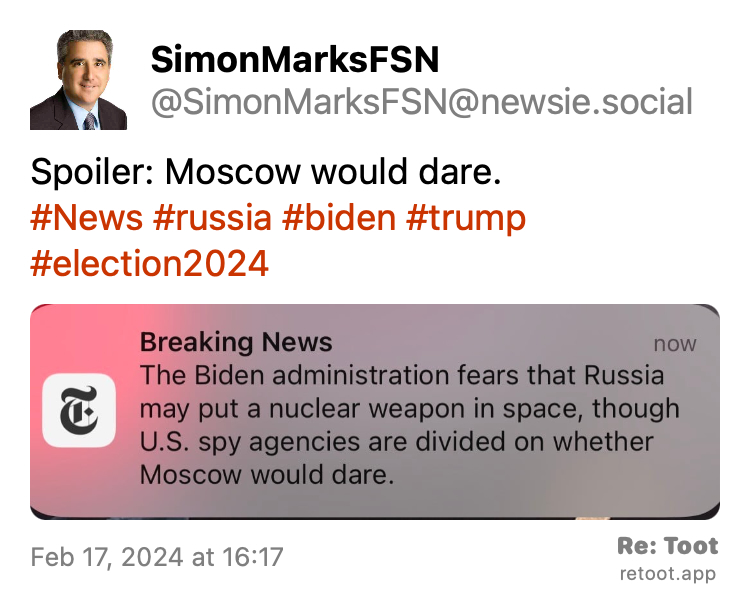
\includegraphics[keepaspectratio]{\%7B\%7Bsite.url\%7D\%7D/img/spacewar.jpg}}
\caption{Post by SimonMarksFSN. ``Spoiler: Moscow would dare. \#News
\#russia \#biden \#trump \#election2024'' The post contains an image
with no description. Posted on Feb 17, 2024 at 16:17}
\end{figure}

\begin{quote}
\emph{Post by SimonMarksFSN. ``Spoiler: Moscow would dare. \#News
\#russia \#biden \#trump \#election2024'' The post contains an image
with no description. Posted on Feb 17, 2024 at 16:17}
\end{quote}

The item highlighted by Simon Marks states: ``The Biden administration
fears that Russia may put a nuclear weapon in space, though U.S. spy
agencies are divided on whether Moscow would dare.''

Things are generally looking quite bad. Despite the idiocy of the MAGA
Party (the old guard of the Republican Party having either been
defenstrated or just walked away), Russia is \emph{not} our friend. The
Russian Federation is still the bad guy. Putin is the bad guy. A nuke
in-orbit is a fabulous way to generate an \emph{EMP}. Such a thing could
easily impact ground-side concerns just as easily as matters space-side.

What could go wrong?

This graphic from DVIDS from 2019
\href{https://www.dvidshub.net/graphic/9655/competing-space-space-based-weapons}{remains
instructive as to the various types of space-based weapons}. There are
more possibilities out there than just nukes.
